%==============================================================================
% Sjabloon poster bachproef
%==============================================================================
% Gebaseerd op document class `a0poster' door Gerlinde Kettl en Matthias Weiser
% Aangepast voor gebruik aan HOGENT door Jens Buysse en Bert Van Vreckem

\documentclass[a0,portrait]{hogent-poster}

% Info over de opleiding
\course{Bachelorproef}
\studyprogramme{toegepaste informatica}
\academicyear{2024-2025}
\institution{Hogeschool Gent, Valentin Vaerwyckweg 1, 9000 Gent}

% Info over de bachelorproef
\title{Leveraging Machine Learning to Examine the Link Between Bitcoin and Tezos Market Dynamics.}
% \subtitle{Ondertitel (eventueel)}
\author{Hanno van Baarle}
\email{Hanno.vanbaarle@student.hogent.be}
\supervisor{Thomas Desmedt}
\cosupervisor{F. J. Kirk}

% Indien ingevuld, wordt deze informatie toegevoegd aan het einde van de
% abstract. Zet in commentaar als je dit niet wilt.
\specialisation{Data-Science \& AI}
% \keywords{Lambda-calculus, Scheme}
% \projectrepo{https://github.com/user/repo}

\begin{document}

\maketitle

\begin{abstract}
This thesis investigates whether short-term Bitcoin (BTC) price dynamics can help predict Tezos (XTZ) price movements, using machine learning. While BTC’s market influence is well established, its predictive power on individual altcoins like Tezos remains underexplored.

To study this, three models—Linear Regression, Random Forest, and XGBoost—were trained on engineered lagged features derived from historical BTC and XTZ data. Model performance was assessed using $R^2$ and Root Mean Squared Error (RMSE).

XGBoost excelled on training data ($R^2 = 0.9948$, RMSE = 0.1117) but showed signs of overfitting ($R^2 = 0.8415$ on test data). Random Forest achieved the best test RMSE (0.0810) and generalization ($R^2 = 0.9182$), though both tree-based models largely ignored BTC-related variables. Linear Regression, while slightly less accurate, revealed meaningful cross-asset dependencies—BTC features such as \texttt{btc\_price\_3d\_ago} were statistically significant, indicating a delayed linear influence from Bitcoin to Tezos.

These findings suggest that while complex models capture autocorrelation well, simpler linear models better expose interpretable, inter-market relationships—critical for understanding and managing volatility in the Tezos ecosystem.
\end{abstract}

\begin{multicols}{3} % This is how many columns your poster will be broken into, a portrait poster is generally split into 2 columns

\section{Introduction}

For Tezos-based decentralized exchanges, such as CrunchySwap, accurately predicting the price of Tezos (\$XTZ) is crucial, as the gas fees required for transaction processing are directly tied to the value of Tezos. Sudden and unpredictable price shifts can lead to operational inefficiencies, higher costs, and user dissatisfaction.

If the price of Tezos drops sharply, gas fees may become disproportionately high relative to the transaction value, increasing costs for users and making the platform less attractive compared to exchanges with more stable fee structures. This could lead to lower transaction volume and reduced user retention. On the other hand, if Tezos' price surges unexpectedly, gas fees may become too low, negatively affecting the platform’s profitability and long-term sustainability.

Given Bitcoin’s influence over the broader cryptocurrency market, understanding its impact on Tezos is critical. Since Bitcoin often dictates market sentiment and liquidity flows, its price movements could serve as leading indicators for Tezos price trends. However, no widely accepted predictive model currently exists to quantify this relationship, leaving Tezos-based exchanges, liquidity providers, and financial analysts with limited tools for managing risk and optimizing fee structures.

\section{Methodology}

The data for this study was sourced from the CoinGecko API and includes historical daily information on Bitcoin and Tezos. 
For both assets, we extracted the date, closing price, trading volume, and market capitalization. 

From these raw features, we engineered lagged variables going back up to five days to capture short-term temporal dynamics. For the Linear Regression model, a StandardScaler was applied to normalize the feature set. Three models were trained: Linear Regression, Random Forest, and XGBoost. 
Their performance was evaluated using the R² score and Root Mean Squared Error (RMSE) on both training and test sets.

\section{Results}

\begin{center}
  \captionsetup{type=figure}
  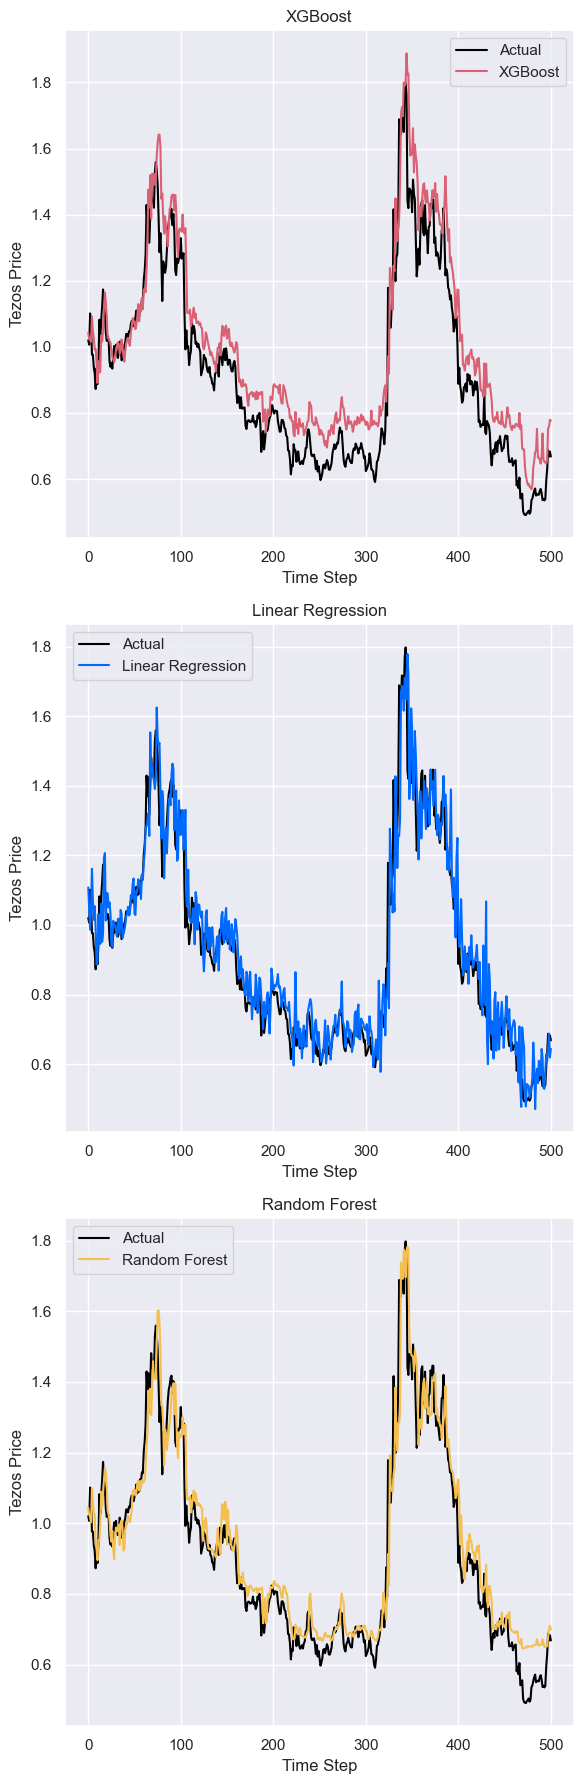
\includegraphics[width=1.0\linewidth]{summaryvert}
  \captionof{figure}{Summary of the three models side by side}
\end{center}

\begin{center}
  \captionsetup{type=figure}
  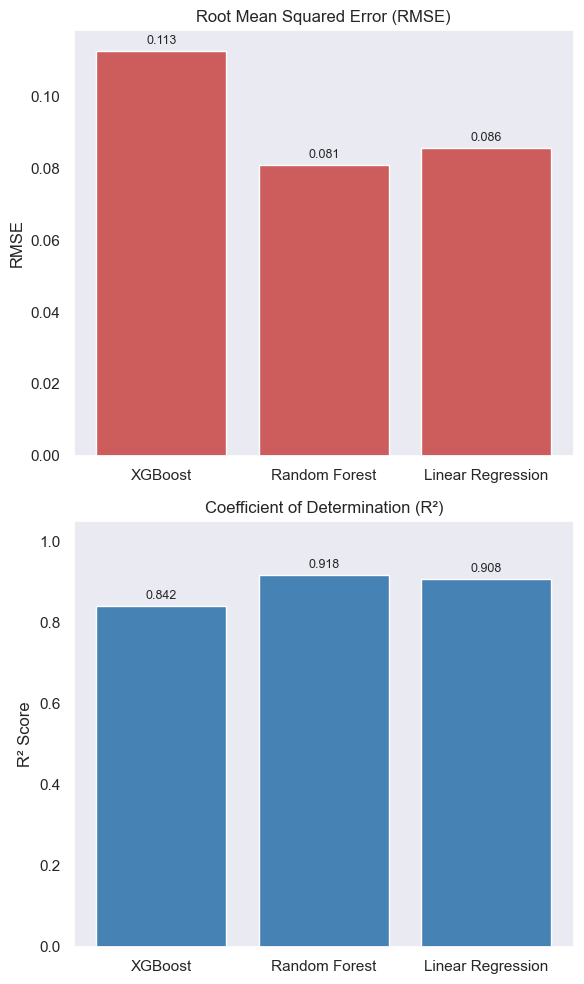
\includegraphics[width=1.0\linewidth]{modelcomparisonvertical}
  \captionof{figure}{Model performance comparison on R² and RMSE}
\end{center}

\section{Conclusions}

While Random Forest and XGBoost achieved high predictive accuracy by focusing on recent Tezos prices, they failed to uncover meaningful relationships with Bitcoin. In contrast, Linear Regression—despite being simpler—identified a statistically significant 3-day lagged influence from Bitcoin market variables. This suggests that interpretability and temporal nuance are crucial when investigating cross-asset dynamics. Predictive performance alone does not imply insight.

\section{Future Research}

Future work should explore richer datasets, such as sentiment analysis, macroeconomic indicators, or on-chain metrics. Testing temporal models like RNNs or transformers may help capture delayed or nonlinear dependencies between cryptocurrencies that our tree-based methods failed to uncover.
\end{multicols}
\end{document}